
\vspace{0.5cm}
\subsubsection{Objectif du Test}
Ce test explore l'impact des variations de débit physique lorsqu'un switch est ajouté entre les deux hôtes. Le lien entre h1 et le switch est limité à 1 Gbit/s pour simuler une contrainte intermédiaire.

\subsubsection{Valeurs Testées}
Pour le lien entre le switch et h2, trois valeurs de débit physique sont appliquées :
\begin{itemize}
    \item 5 \% de la valeur par défaut de 2.5 Gbit/s (soit 125 Mbit/s).
    \item 25 \% de la valeur par défaut de 2.5 Gbit/s (soit 625 Mbit/s).
    \item La valeur par défaut de 2.5 Gbit/s.
\end{itemize}
\begin{figure}[h]
    \centering
    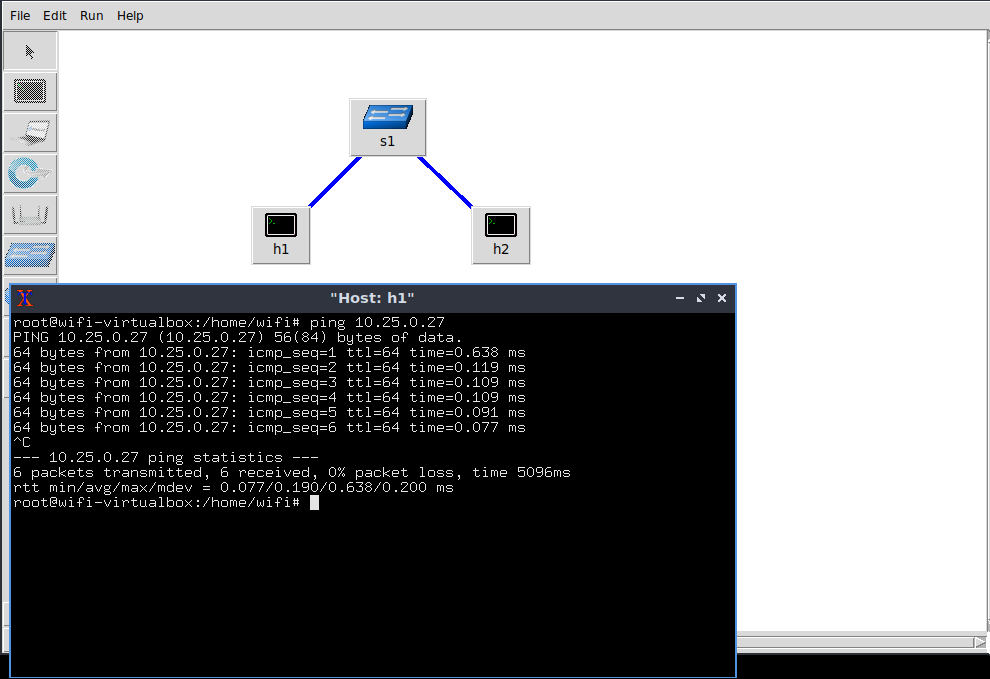
\includegraphics[width=1\textwidth]{./images/T1.2TopologyAndPing.png}
    \caption{Commande ping pour la topologie 2}
    \label{fig:exemple}
\end{figure}

\newpage
\textbf{1:`Debit physique 125Mbit/s`} 
\begin{figure}[H]
    \centering
    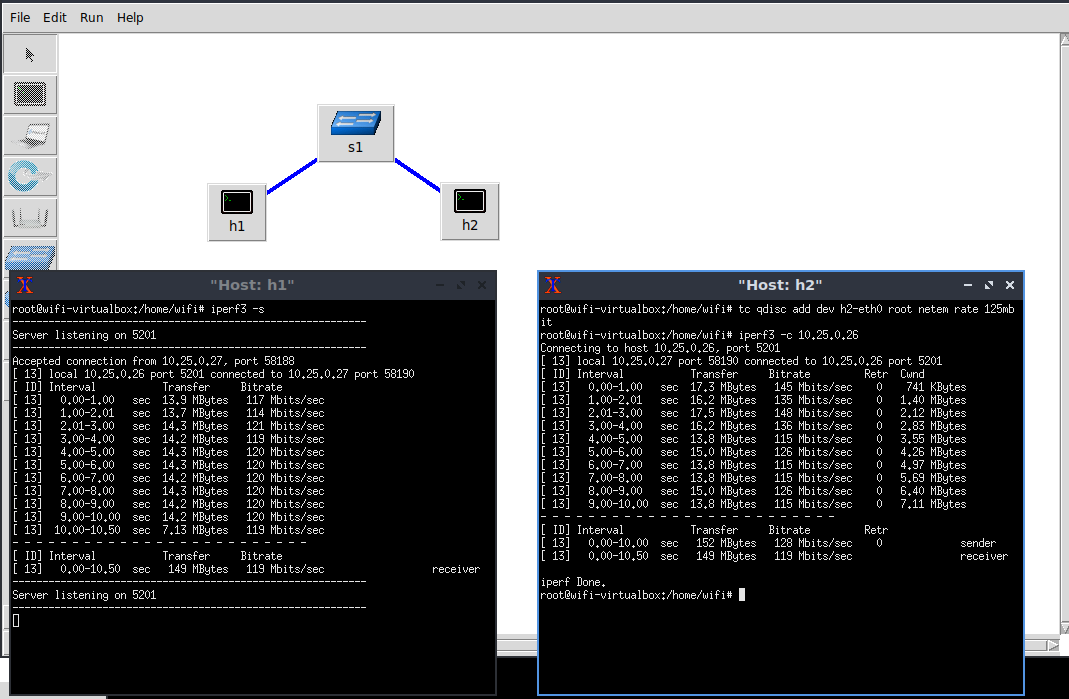
\includegraphics[width=0.85\textwidth]{./images/T1.2/125test2.png}
    \caption{Test2 pour debit physique = 125Mbit/s}
    \label{fig:exemple}
\end{figure}
\begin{figure}[H]
    \centering
    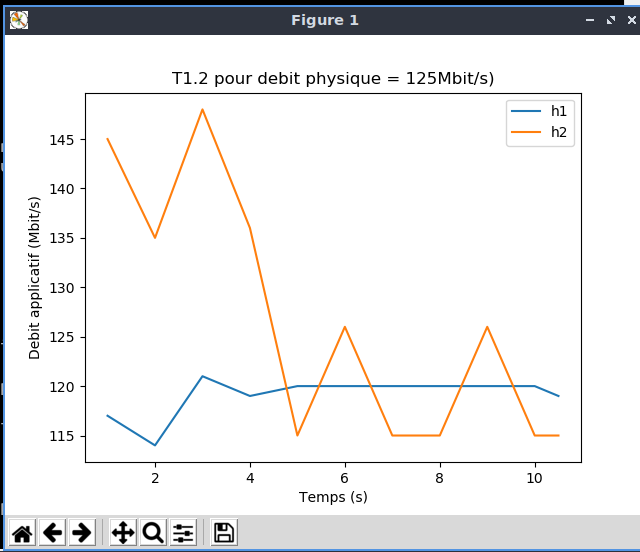
\includegraphics[width=0.85\textwidth]{./images/T1.2/courbe125test2.png}
    \caption{Graphe du test2 pour debit physique = 125Mbit/s}
    \label{fig:exemple}
\end{figure}

\textbf{Observation :}\\
Débit de H1 (ligne bleue) : Le débit applicatif mesuré sur h1 reste relativement stable, oscillant entre 115 Mbit/s et 125 Mbit/s tout au long du test. Même si le lien physique entre H1 et le switch est de 1 Gbit/s, le débit observé n’atteint jamais cette valeur maximale théorique.

Débit de H2 (ligne orange) : Le débit applicatif de H2 fluctue considérablement, atteignant parfois des pics autour de 145 Mbit/s, mais chutant aussi à des valeurs proches de 120 Mbit/s ou même légèrement en dessous.
\vspace{1cm}
\\
\textbf{Explications :} 
\\
Bien que la liaison entre h1 et le switch soit fixée à 1 Gbit/s, c'est le lien entre H2 et le switch qui impose une limite plus contraignante de 125 Mbit/s.\\
Dans ce type de configuration, le débit total du transfert est dicté par le maillon le plus faible de la chaîne, en l’occurrence la connexion limitée entre H2 et le switch. Le lien de 1 Gbit/s entre h1 et le switch ne peut donc pas être exploité pleinement tant que H2 ne peut pas recevoir ou envoyer des données plus rapidement que 125 Mbit/s.\\
\\
L'outil iperf3 utilise généralement le protocole TCP, qui ajuste automatiquement le débit en fonction des capacités du réseau. TCP surveille les capacités des deux hôtes et ajuste son débit en fonction des retours qu’il reçoit (accusés de réception des paquets).
Ici, TCP détecte que le débit sur le lien entre H2 et le switch est limité à 125 Mbit/s et ajuste donc la transmission des données pour s’adapter à cette contrainte, expliquant pourquoi le débit de h1 reste autour de 115 à 125 Mbit/s.
Le protocole TCP est conçu pour éviter la surcharge du réseau et s’adapte dynamiquement aux conditions de congestion, ce qui pourrait aussi expliquer pourquoi le débit de H2 est plus instable, car le lien est proche de sa capacité maximale.\\
\\
\textbf{2:`Debit physique 625Mbit/s`} 
\begin{figure}[H]
    \centering
    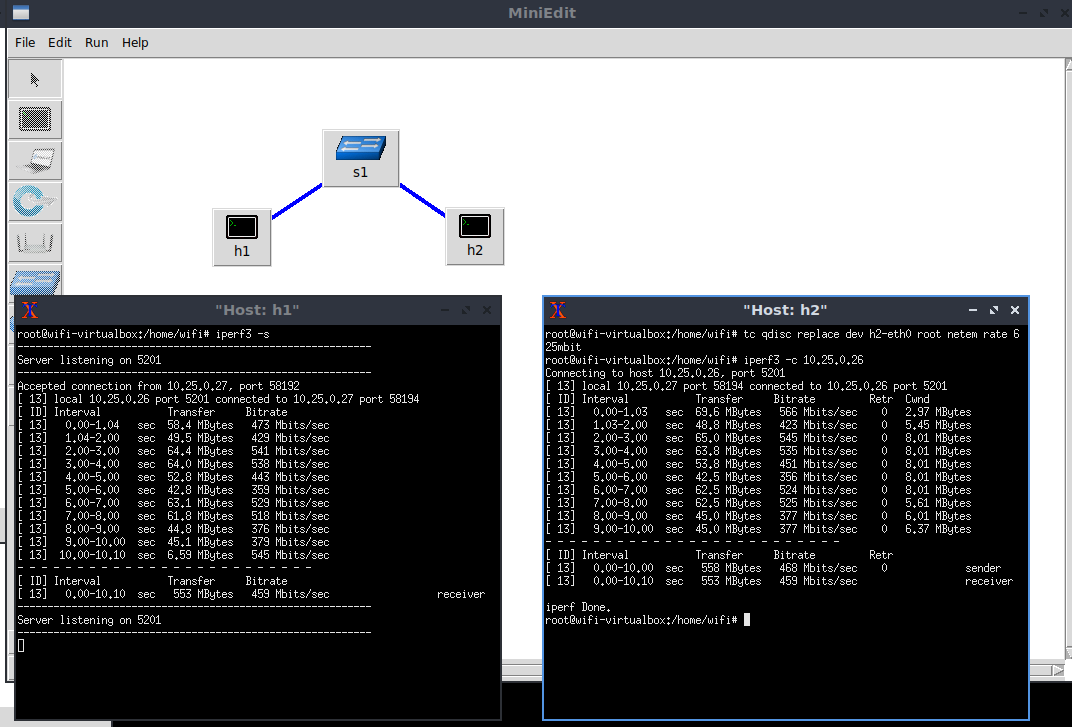
\includegraphics[width=0.7\textwidth]{./images/T1.2/625test2.png}
    \caption{Test2 pour debit physique = 625Mbit/s}
    \label{fig:exemple}
\end{figure}
\begin{figure}[H]
    \centering
    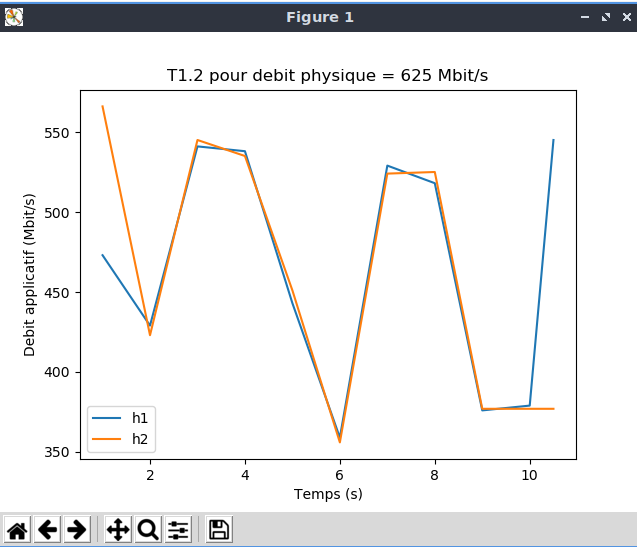
\includegraphics[width=0.8\textwidth]{./images/T1.2/courbe625test2.png}
    \caption{Graphe du test2 pour debit physique = 625Mbit/s}
    \label{fig:exemple}
\end{figure}

\textbf{Observation :}\\
Débit de h1 (ligne bleue) : Le débit applicatif mesuré sur h1 varie entre 350 Mbit/s et environ 550 Mbit/s.
Débit de h2 (ligne orange) : Le débit applicatif sur H2 suit une courbe similaire à celle de h1.
\\
\\
\textbf{Explication} :\\
Le fait que les deux débits (h1 et h2) suivent un schéma similaire de montée et descente suggère que la limitation du débit physique à 625 Mbit/s entre H2 et le switch influence directement les deux hôtes. Comme le débit de H2 est limité par le lien physique, le switch agit comme un point de congestion, entraînant des fluctuations du débit applicatif.
\vspace{1cm}
\\
\newpage
\textbf{3:`Debit physique 2.5Gbit/s`} 
\begin{figure}[H]
    \centering
    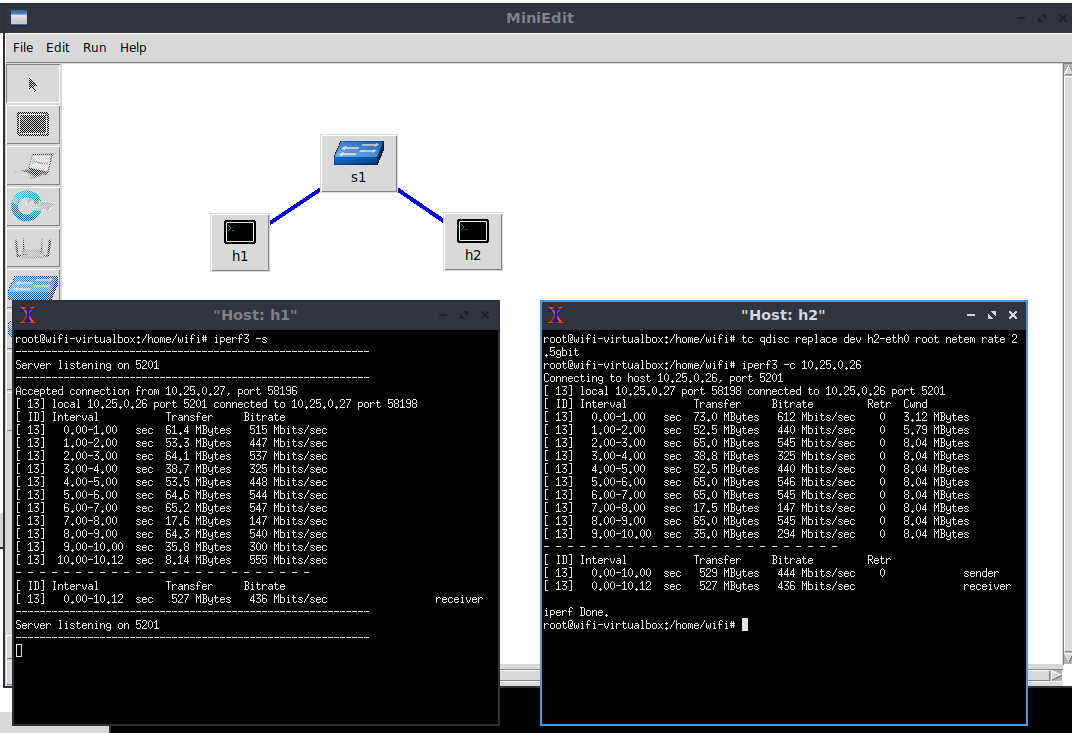
\includegraphics[width=0.8\textwidth]{./images/T1.2/2500test2.png}
    \caption{Test2 pour debit physique = 2.5Gbit/s}
    \label{fig:exemple}
\end{figure}
\begin{figure}[H]
    \centering
    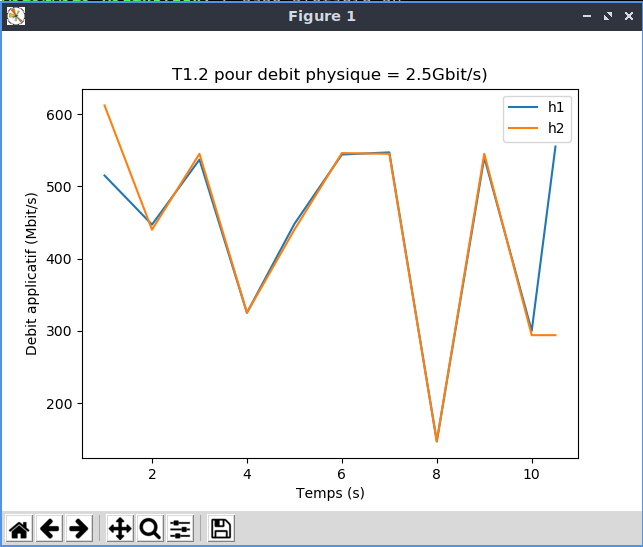
\includegraphics[width=0.8\textwidth]{./images/T1.2/courbe2500test2.png}
    \caption{Graphe du test2 pour debit physique = 2.5Gbit/s}
    \label{fig:exemple}
\end{figure}

\textbf{Explication} :\\
Le débit applicatif oscille de manière significative entre environ 100 Mbit/s et 600 Mbit/s sur la période mesurée (10 secondes).
\\

Les courbes de h1 et h2 sont très proches, ce qui indique une synchronisation des débits mesurés sur les deux hôtes.`\\
Le fait de fixer le débit de l'interface h2 à 2.5 Gbit/s alors que le lien entre h1 et le switch est limité à 1 Gbit/s signifie que le débit maximum théorique du transfert sera contraint par cette limite de 1 Gbit/s.
\\
\\Toutefois, les fluctuations observées montrent que le débit applicatif est souvent bien en-dessous de ce maximum théorique, probablement en raison des phénomènes de contention et de gestion des files d'attente (dqisc).
\vspace{0.5cm}
\\
Si le lien entre h1 et le switch est limité à 1 Gbit/s, alors que le lien entre h2 et le switch peut aller jusqu'à 2.5 Gbit/s, il y a un déséquilibre.
Lorsqu'h2 essaie d'envoyer des données à un débit supérieur à 1 Gbit/s, le switch doit gérer cette surcharge, créant ainsi une contention pour la bande passante disponible.
\\
En présence de forte contention, des collisions peuvent se produire (particulièrement sur les réseaux partagés comme Ethernet en mode half-duplex).
Les paquets peuvent être perdus et doivent être retransmis, ce qui réduit l'efficacité du débit applicatif.\\
\\
\textbf{4:`Explication du Graphique Débit Applicatif vs Débit Physique`}
\begin{figure}[H]
    \centering
    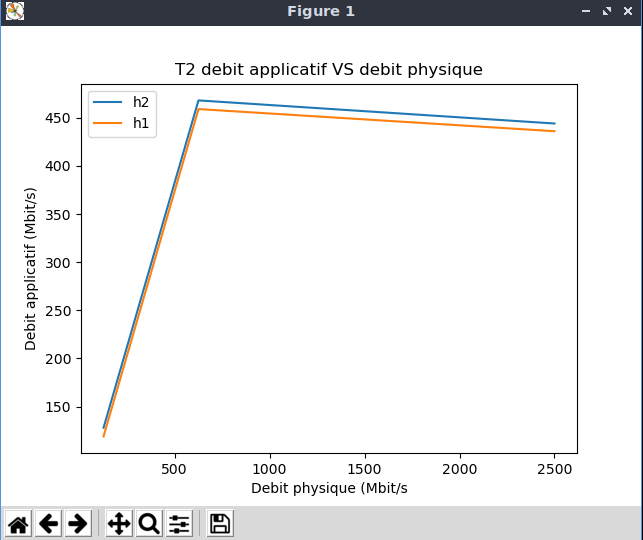
\includegraphics[width=0.8\textwidth]{./images/T1.2/T2appVSphy.png}
    \caption{Graphe du test2 pour Débit Applicatif vs Débit Physique}
    \label{fig:exemple}
\end{figure}
\newpage
\textbf{Explication} :\\
Le graphique montre une relation linéaire entre le débit physique et le débit applicatif pour les valeurs de 125 Mbps, 625 Mbps et 2,5 Gbps.  L’allure du graphe suggère une certaine saturation des performances applicatives à mesure que le débit physique augmente au-delà de la capacité de transfert maximale permise par le lien entre le switch et H1.
La cause de ce phénomène est la limitation imposée par le débit du lien entre le switch et H1, qui reste fixe à 1 Gbit/s tout au long du test. Même lorsque le débit physique au-delà de ce lien (entre H2 et le switch) est augmenté, le débit applicatif ne peut dépasser cette limite. Cela signifie que le débit applicatif est contraint par le débit maximal autorisé sur le lien entre le switch et H1. En d’autres termes, une fois un certain seuil atteint, augmenter davantage le débit physique ne se traduit pas par une amélioration du débit applicatif, car le goulot d'étranglement est situé au niveau du lien entre le switch et H1.